\clearpage
\section{Background for Discussion (not part of the submission)}\label{app:meeting}

This section collects implementation details and run diagnostics for discussion among the authors. Unless stated otherwise, the statistics are medians over the 36 configurations solved by Standard BD (instances p4, p5, p10 and p50 with 100, 300 and 500 scenarios).

\subsection{Gurobi Settings}\label{app:gurobi}

Table~\ref{tab:gurobi} lists the Gurobi~12.0.0 parameters that matter for single-tree Benders, their meaning, the Gurobi default, typical choices in the literature, and our setting. Parameters not listed are at their defaults (e.g., \texttt{Presolve}, \texttt{MIPFocus}, \texttt{Cuts}, \texttt{Heuristics}=0.05, \texttt{Seed}=0, \texttt{FeasibilityTol}=\texttt{OptimalityTol}=$10^{-6}$, \texttt{IntFeasTol}=$10^{-5}$). The scenario subproblems are LPs solved with default settings and \texttt{OutputFlag}=0; the master problem prints its log.

\begin{table}[h]
\centering
\caption{Gurobi parameters of the master MIP.}\label{tab:gurobi}
\scriptsize
\setlength{\tabcolsep}{3pt}
\begin{tabular}{p{2.1cm}p{4.3cm}p{1.2cm}p{2.2cm}p{1.6cm}}
\toprule
Parameter & Meaning & Default & Common choices & Ours\\
\midrule
\texttt{LazyConstraints} & must be 1 to add constraints with \texttt{cbLazy} at integer candidates (\texttt{MIPSOL}); disables reductions that could cut off solutions & 0 & 1 in every single-tree Benders code & 1\\
\texttt{MIPGap} & stop when $(UB-LB)/|UB|$ is below this value & $10^{-4}$ & $10^{-4}$ (default), $10^{-3}$ or $10^{-2}$ in Benders studies & $10^{-3}$\\
\texttt{TimeLimit} & wall-clock limit in seconds & $\infty$ & 1--3 h; 3 h (10\,800 s) is frequent & 10\,800\\
\texttt{Threads} & number of threads (0 = all cores) & 0 & equal to the allocated cores & 16 (via \texttt{gurobi.env})\\
\texttt{PreCrush} & lets presolve translate user cuts added with \texttt{cbCut} at \texttt{MIPNODE}; Gurobi asks for 1 when adding user cuts & 0 & 1 when \texttt{cbCut} is used & 0 (not set)\\
\texttt{OutputFlag} & solver log on/off & 1 & 1 for the master, 0 for subproblems & 1 / 0\\
\texttt{Method} & LP algorithm ($-1$ automatic, 0 primal, 1 dual simplex, 2 barrier) & $-1$ & dual simplex for repeated subproblem LPs & $-1$\\
\bottomrule
\end{tabular}
\end{table}

Cuts are added at integer candidates with \texttt{cbLazy} (callback \texttt{MIPSOL}) and at fractional nodes with \texttt{cbCut} (callback \texttt{MIPNODE}, only when the node LP is optimal). The Gurobi logs report all retained Benders cuts as ``Lazy constraints'' and no ``User'' cuts; whether the \texttt{cbCut} cuts are used without \texttt{PreCrush}=1 is worth checking, because it affects all methods equally.

\subsection{Data Generation}\label{app:datagen}

The scenario files are produced by \texttt{SCFLP\_data\_generation\_version4.py} (method \texttt{merve\_with\_covariate\_with\_random\_demand\_capacity}, NumPy \texttt{default\_rng} with seed 42 for every file), starting from the corrected reading of the Holmberg instances (capacity and fixed cost per facility, unit cost $c_{ij}/\bar d_i$).
\begin{enumerate}
\item \emph{Capacity scenarios.} For each facility, $\sigma^u_j\sim U(0.1u_j,0.3u_j)$; scenario 1 keeps $u_j$, and scenarios $2,\dots,S$ draw $u_{j,m}\sim\mathcal N(u_j,(\sigma^u_j)^2)$, clipped at zero.
\item \emph{Demand scenarios.} For each customer, $\sigma_i\sim U(0.1\bar d_i,0.3\bar d_i)$, and $d_{i,m}=\max\{0,D_{i,m}\}$ with $D_{i,m}\sim\mathcal N(\bar d_i,\sigma_i^2)$. If $\sum_i d_{i,m}$ exceeds the total capacity of scenario $m$, all demands of the scenario are multiplied by 0.9 until it does not.
\item \emph{Covariates.} The scenario matrix $[\mathbf d_m,\mathbf u_m]_{m}$ is centred, and the first six left singular vectors of its SVD give six PCA covariates per scenario.
\item \emph{Predictability diagnostics.} For each customer (and facility), the demand (capacity) is predicted from the covariates with linear regression, $k$-NN ($k=2$), $k$-means clustering (up to 10 clusters) and a regression tree on an 80/20 split; the training $R^2$, test MSE and test MAPE are written to the \texttt{\# Diagnostics} block of the file.
\end{enumerate}
The runs use \texttt{use\_stochastic\_capacity}=False and \texttt{use\_covariates}=\texttt{features\_only} (VERIFIED in all 105 solution logs): the stored capacity scenarios and covariates are not used by the solver or by LABD, the second stage uses the base capacities $u_j$, so $\mathbf T_m=\mathbf T$, and relatively complete recourse is enforced by the master constraint $\sum_ju_jx_j\ge\max_m\sum_id_{i,m}$.

\subsection{What Happens Inside the Runs}\label{app:runstats}

Table~\ref{tab:runstats} and Fig.~\ref{fig:diag} report how the solve proceeds. A \emph{callback} is one cut-generation round, at an integer candidate or at a fractional node. \emph{Integer candidates} are the \texttt{MIPSOL} callbacks, i.e., integer master solutions submitted to the callback, most of which are cut off. \emph{Cuts generated} counts the cuts built from exact and from predicted (or averaged) duals; \emph{cuts in master} is the number of lazy constraints Gurobi keeps at the end.

\begin{table}[h]
\centering
\caption{Median run statistics on the configurations solved by Standard BD (times in seconds).}\label{tab:runstats}
\scriptsize
\setlength{\tabcolsep}{3pt}
\begin{tabular}{lrrrrrrrrr}
\toprule
Method & Time & Warm-up & $p$-median & Callbacks & B\&B nodes & Int.\ cand. & \multicolumn{2}{c}{Cuts generated} & Cuts in master\\
\cmidrule(lr){8-9}
 & & & & & & & exact & predicted & \\
\midrule
Standard BD & 762 & -- & -- & 291 & 298 & 76 & 71\,615 & -- & 15\,651\\
LABD 5\% & 82 & 15 & 0.5 & 280 & 300 & 85 & 4\,694 & 70\,170 & 18\,865\\
LABD 15\% & 156 & 14 & 4.6 & 293 & 304 & 77 & 11\,060 & 57\,006 & 15\,508\\
LABD 25\% & 233 & 14 & 8.2 & 271 & 275 & 81 & 18\,166 & 51\,499 & 16\,565\\
RND 5\% & 230 & -- & -- & 1\,275 & 923 & 484 & 11\,354 & 110\,211 & 40\,218\\
RND 15\% & 416 & -- & -- & 1\,110 & 897 & 390 & 26\,487 & 114\,182 & 41\,609\\
RND 25\% & 518 & -- & -- & 978 & 748 & 378 & 35\,088 & 82\,169 & 34\,931\\
\bottomrule
\end{tabular}
\end{table}

\begin{figure}[h]
\centering
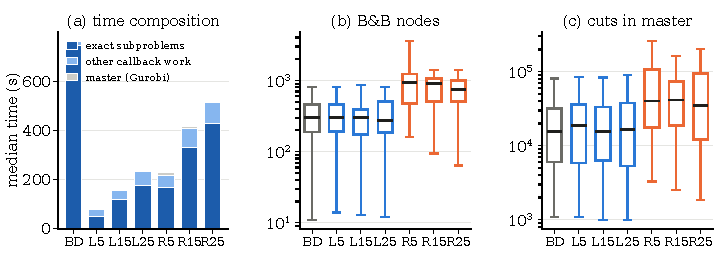
\includegraphics[width=\textwidth]{figures/fig_diag.pdf}
\caption{(a) Median solution time split into exact subproblem solves, other callback work (prediction, certification, selection, cut construction) and the master MIP. (b) Branch-and-bound nodes and (c) Benders cuts retained in the master, log scale. BD: Standard BD; L5--L25: LABD with 5--25\% exact share; R5--R25: RND.}\label{fig:diag}
\end{figure}

Three observations follow.
\begin{itemize}
\item \emph{LABD follows the same search as Standard BD.} It needs about the same number of callbacks (about 280 versus 291), nodes and integer candidates, and keeps a similar number of cuts. Each callback is cheaper because only the $p$ representative subproblems are solved exactly: exact subproblem time drops from about 743~s to 49--201~s.
\item \emph{RND searches much more.} With averaged duals of random subproblems, its cuts are weaker: it needs 3--4 times more callbacks and 2.5--3 times more nodes, submits about five times more integer candidates (most cut off), and keeps 2--3 times more cuts in the master. This is why it is not faster despite solving the same number of subproblems exactly.
\item \emph{Fixed costs of LABD.} Warm-up takes about 15~s (all subproblems solved exactly for five rounds), and the $p$-median selection grows with the share (median 0.5~s at 5\%, 8~s at 25\%, up to 210~s on p4 with 500 scenarios). Training, prediction, certification and the guard together take a few seconds. About 73\% of the raw predictions are infeasible and are certified.
\end{itemize}

\subsection{Bounds over Time}\label{app:lbub}

Fig.~\ref{fig:lbub} plots the lower bound (LB, best bound of the master) and the upper bound (UB, incumbent of the master) recorded in every callback, together with the master gap $(UB-LB)/UB$, for a typical instance (p4, 500 scenarios) and for p10 with 300 scenarios. For Standard BD both bounds refer to the true problem. For LABD and RND they refer to the \emph{surrogate} master built with predicted or averaged cuts: the run stops when the surrogate gap is below $0.1\%$, and the returned solution is then evaluated exactly. The dotted line is the optimal objective.

\begin{figure}[h]
\centering
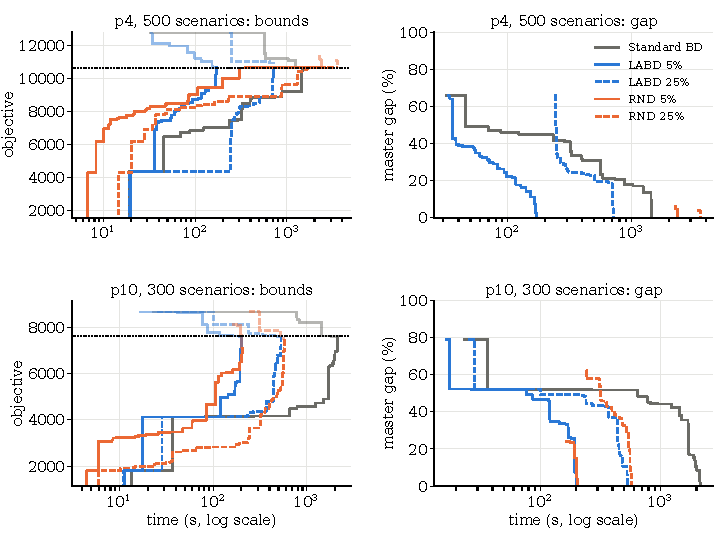
\includegraphics[width=\textwidth]{figures/fig_lbub.pdf}
\caption{Master lower bound (rising curves) and upper bound (lighter falling curves), and master gap, over time. Solid: 5\% exact share; dashed: 25\%.}\label{fig:lbub}
\end{figure}

\begin{itemize}
\item On p4, LABD closes the gap in 171~s at 5\% and 717~s at 25\%, against 1\,465~s for Standard BD. Its bounds follow the same pattern as those of Standard BD, compressed in time.
\item RND raises its lower bound quickly, but it finds no incumbent for a long time: Gurobi keeps proposing integer solutions and the callback keeps cutting them off with new averaged cuts. On p4 its first incumbent appears only after about 2\,265~s at 5\% (Standard BD and LABD have one after about 30~s), which is why its total time exceeds that of Standard BD.
\item On p10 with 300 scenarios, RND at 5\% is as fast as LABD, but its surrogate stops at a bound of 7\,093, far below the optimum 7\,611: its averaged cuts underestimate the recourse, and the returned solution is $1.56\%$ worse than optimal. LABD stops at 7\,603, just below the optimum, and returns the optimal solution.
\end{itemize}

\subsection{Reading a Gurobi Log}\label{app:gurobilog}

The folder \texttt{logs/} of this repository contains the Gurobi logs of the master problem for p10 with 300 scenarios (Standard BD, LABD 5\%, RND 5\%). The main parts of the Standard BD log are as follows.

\begin{enumerate}
\item \emph{Header.} \texttt{Read parameters from file gurobi.env} sets \texttt{Threads}=16; then \texttt{LazyConstraints}, \texttt{MIPGap} and \texttt{TimeLimit} are set by the code, and the block ``Non-default parameters'' confirms them.
\item \emph{Model.} \texttt{Optimize a model with 2 rows, 310 columns}: the master starts with only the capacity constraint (plus one constraint presolve removes), 10 binary facility variables and 300 continuous recourse variables $\eta_m$; all Benders cuts are added later through the callback.
\item \emph{Root relaxation.} Objective 1\,800: without any cut the $\eta_m$ can be zero, so the first bound is the LP bound on the fixed costs alone. Benders cuts raise it during the search.
\item \emph{Node log.} Each line reports explored and unexplored nodes, the node objective and depth, the number of fractional variables (\texttt{IntInf}), the incumbent, the best bound (\texttt{BestBd}), the gap, simplex iterations per node and elapsed time. A line starting with \texttt{H} is an incumbent found by a heuristic, and \texttt{*} an incumbent found at a node; both must first survive the lazy-cut check in the callback.
\item \emph{Cut summary.} \texttt{Cutting planes: Lazy constraints: 44701} is the number of Benders cuts retained in the master. No ``User'' cuts are listed, although the trace records about 143\,000 cuts submitted with \texttt{cbCut} at fractional nodes; this supports the \texttt{PreCrush} question in Appendix~\ref{app:gurobi}.
\item \emph{Termination.} \texttt{Explored 745 nodes \ldots\ in 2149.39 seconds}, \texttt{Optimal solution found (tolerance 1.00e-03)}, best objective and bound 7\,611.37. The last line, \texttt{User-callback calls 2694, time in user-callback 2138.32 sec}, shows that 99.5\% of the time is spent in the callback, i.e., in solving subproblems and building cuts; the master MIP itself takes about 11~s.
\end{enumerate}

The LABD and RND logs read the same way. Their ``best objective'' is the surrogate value (7\,603 for LABD, 7\,093 for RND), not $V(\widehat{\mathbf x})$; LABD spends 195 of its 201~s in the callback, and RND 198 of 205~s.
